% File: basic_elements.tex
\documentclass{standalone}
\usepackage[american]{circuitikz}
\usepackage{cmbright}

\definecolor{myred}{RGB}{170,0,0}
\definecolor{myblue}{RGB}{0,0,220}

\ctikzset{bipoles/resistor/height=0.2}
\ctikzset{bipoles/resistor/width=0.5}

\begin{document}
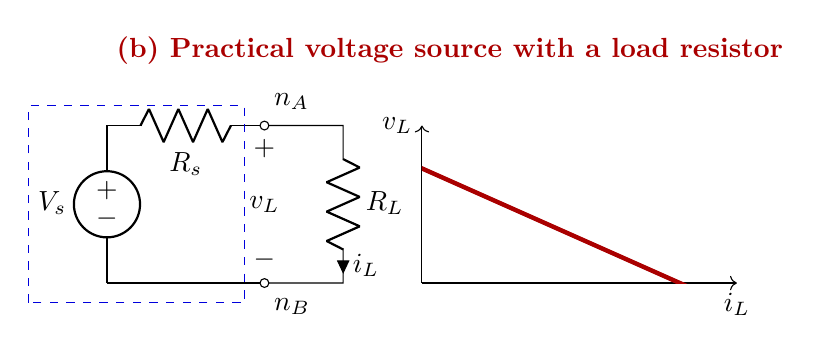
\begin{tikzpicture}
    % Subtitle for the circuit.
    \node[anchor=north west, font=\bfseries, color=myred] at (0, 3.25) {(b) Practical voltage source with a load resistor};
    % --- Circuit (top left)
    \begin{scope}
        % Nodes A and B
        \draw (2, 2) node[ocirc] (A) {};
        \draw (A) node[right, yshift=3mm] {$n_A$};
        \draw (2, 0) node[ocirc] (B) {};
        \draw (B) node[right, yshift=-3mm] {$n_B$};

        % Voltage source and lower wire
        \draw (0, 0) to[V, l={$V_s$}, invert] (0, 2) to[R, l_=$R_s$] (A);
        \draw (0, 0) -- (B);

        % Resistor and upper wire
        \draw (A) to ++(1, 0)
            to[R, l=$R_L$, i^>=$i_L$] ++(0, -2)
            to (B);

        % Voltage label across A and B
        \draw (A) to[open, v^=$v_{L}$] (B);

        % Dotted box around the ideal source circuit
        \draw[dashed, thin, myblue] (-1.0, -0.25) rectangle (1.75, 2.25);
    \end{scope}

    % Plot of v_L vs i_L (top right)
    \begin{scope}[xshift=4cm]
        % Axes
        \draw[->] (0, 0) -- (0, 2) node[left] {$v_L$};
        \draw[->] (0, 0) -- (4, 0) node[below] {$i_L$};
        % Plot
        \begin{scope}
            % vl = v_s - i_L * R_s
            \clip (0, 0) rectangle (4, 2);
            \draw[ultra thick, myred] (-0.1, 1.5) -- (3.5, -0.1);
        \end{scope}
    \end{scope}
\end{tikzpicture}
\end{document}